\documentclass[12pt,a4paper]{article}
\usepackage{graphicx}
\usepackage{biblatex}
\usepackage{parskip}
\usepackage{listings}
\usepackage{pdfpages}

\lstset{%
basicstyle=\ttfamily,
breaklines = true,
tabsize=2
}
\graphicspath{ {./Images/} }
\addbibresource{biblography.bib}

\setlength{\parskip}{1em}
\begin{document}

\begin{titlepage}
	\newcommand{\HRule}{\rule{\linewidth}{0.5mm}}
    
\includegraphics[width = 4cm]{./Images/Logo.jpg}\\[0.5cm] 
    
    \center 
	\textsc{\large Department of Electrical and Electronic Engineering }\\[0.5cm] 
	\textsc{\normalsize ELEC40006: Electronics Design Project}\\[0.5cm] 
    
	\HRule \\[0.4cm]
	Circuit Simulator Technical Report
    \HRule \\[1.5cm]
     
    \begin{center}
		Authors:\\[0.5cm] Xin Wang\\CID: 01735253\\xin.wang19@imperial.ac.uk \\[0.5cm]
		Brandon Cann\\ CID: 01724765\\ brandon.cann19@imperial.ac.uk\\[0.5cm]
		Adam Rehman\\ CID: \\adam.rehman19@imperial.ac.uk\\[0.5cm]
	\end{center} \large
    
    \vfill % Fill the rest of the page with whitespace
 	\small Submitted in partial fulfillment of the requirements for ELEC40006 \\ [0.5cm]
    \makeatletter
    \@date 
    \makeatother
\end{titlepage}

\tableofcontents
\pagebreak

\section{Overview of the report}
This report loosely follows the stages of the Software Developement Cycle. \par
Section 2 details the design problem presented and the program requirements at are necessary for a preliminary design 
to be established. \par
Section 3 provides a summary of the program development timeline and the details relating to project management format
the format of meeting minutes used to how the responsibilities are distributed among the project team. \par
Section 4 discusses the preliminary designs produced by the team and the rationale behind some design choices implemented
by the team. \par
Section 5 gives an comprehensive overview of the program design, detailing the functions and flowcharts used. \par 
Section 6 investigates the design constraints of the program, the accuracy of the results produced and the speed of 
execution as the circuit size varies.\par
Section 7 serves as a continuation of Section 6, discussing the possible improvements to mitigate problems encountered
during testing. \par
Section 8 details the possible features that can be added on to the existing program and the required modifications to the
program to add the mentioned features.
\pagebreak

\section{Project Specification}
	\subsection{Design Problem}
	Develop a program that is able to read in a file describing a circuit specified by the user, perform 
	transient simulation on that circuit and output the calculated voltages at each instance in time into a file. 
	\subsection{Program Requirements}
	The main program requirements are listed as follows:
	\begin{itemize}
		\item Program must support basic circuit components listed as follows \footnote{Advanced component can be supported
		provided development schedule is not constrained.}:
		\begin{itemize}
			\item Resistors
			\item Ideal Capacitors
			\item Ideal Inductors
		\end{itemize}
		\item Input file must adhere to SPICE netlist formats
		\item The output file must be in Comma Separated Value (.CSV) format.
		\begin{itemize}
			\item Columns of output file represent nodes in the circuit.
			\item Rows of output file represent an instance in the simulation.
		\end{itemize}
	\end{itemize}
	\pagebreak
	\subsection{Design Criteria}
	The team has identified several factors from the list given in the Product Design Specification document.
	\begin{itemize}
		\item Maintenance: One of the most important factors the team identified. As the development timescale is 
		constrained and the features required is open-ended, so it is important we ensure the design can 
		incorporate new features efficiently and cost-effectively if the client wishes to add new features.
		\item Documentation: For a non-intuitive program, proper documentation is required for client and future
		programmers to make modifications should the client wish.
		\item Performance: No strict performance guidelines are given by the client but the execution 
		speed should still be reasonable. 
		\item Time scale: 6 weeks with a definite deadline. It is important to balance proper team management
		techniques and creating a program that meets client standards.
		\item Testing: Numerous test programs have been created to test various aspects of the program to ensure
		accurate results have been produced. The results produced have been verified with LTSpice, a well 
		established circuit simulation program.
		\item Patents: SPICE engine is a public domain software so we could possibily utilise the engine.
		\item Ergonomics: A Graphics User Interface (GUI) is not specified by the client and could possibly 
		make the program much easier to use.
	\end{itemize}
	\vfill
	\pagebreak

\section{Team Management}
	\subsection{Project timeline overview}
	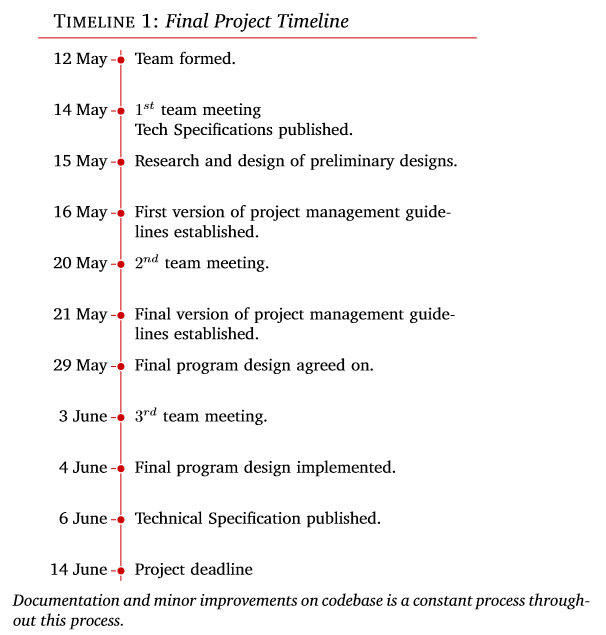
\includegraphics{Timeline.PNG}
	\pagebreak

	\subsection{Gnatt chart}
	\pagebreak

	\subsection{Management approach}
	The project team, with research on different forms of project management, decided on using a Waterfall project
	management approach. The phases are listed as follows: \par
	\begin{itemize}
		\item System and Software Requirements.
		\item Analysis.
		\item Design.
		\item Coding.
		\item Testing.
	\end{itemize}
	This method is selected mainly since the project is short, requirements are clear and the team 
	is not constantly required to report to the client at the early stages of the software development to ensure 
	client statisfaction. \par

	The Waterfall methodology prioritises proper documentation throughout the whole development process. This is important
	to the team as the team project requires a Project Report to be submitted and, due to the ongoing remote lab orals and 
	family-related obligations during quarantine, allows a team member to be quickly caught up should a member step out
	of the team for a while.  

	The disadvantage of the Waterfall methodology lies mainly in that no working software is produced until late in the 
	cycle so there is a level of risk and uncertainty with not being able to meet the deadline, especially in the 
	current state of the world \footnote{Any unforseen circumstances are listed in team meeting minutes summarised the following sections.}. 
	The project team later realised the methodology is not exactly suitable for the Object Orientated Approach 
	that the team eventually settled on. As the integration is done at the end, there is a possibility that any errors
	in the program is not caught during integration.

	\vfill
	\pagebreak

	\subsection{Team responsibilities breakdown}
	The responsibilities of each team member is discussed during the 1st meeting and formalised in the 2nd meeting. The
	respective roles are partly determined by the Belbin questionnaire provided by Mrs. Perea 
	\footnote{Belbin questionnaire forms are found in Appendix: Belbin Roles.}
	\par
	The main responsibilities of each team member is listed as follows:
	\begin{itemize}
		\item Adam Rehman
		\begin{itemize}
			\item Plant
			\begin{itemize}
				\item Research program.
				\item Coding the program.
				\item Testing program.
			\end{itemize}
		\end{itemize}
		\item Brandon Cann
		\begin{itemize}
			\item Monitor Evaluator
			\begin{itemize}
				\item Ensure documentation managed by Xin Wang and coding managed by Adam is in sync.
				\item Contributes to program aspects that is falling behind.
				\item Ensure project requirements are met.
			\end{itemize}
		\end{itemize}
		\item Xin Wang
		\begin{itemize}
			\item Implementer
			\begin{itemize}
				\item Creating and managing the team Project Report and various other documentations.
				\item Meeting minute keeper.
				\item Ensuring code written is up to a standard format with proper comments.
				\item Manages repository base.
			\end{itemize}
		\end{itemize}
	\end{itemize}

	\vfill
	\pagebreak

	\subsection{Project meeting minutes}
	The meeting minutes follow a standard template that is attached under Appendix: Meeting Minutes. \par
	There is no standard protocol for calling team meetings, team meeting are called usually when there is a problem
	that is applicable to all team members. Usually, there is informal communication across various channels from 
	WhatsApp to Discord. \par
	Over the course of the development cycle, there has been three formal meetings and the main reasons and conclusions
	are listed below.
	\begin{itemize}
		\item Meeting 1
		\begin{itemize}
			\item Reason: 
			\begin{itemize}
				\item Project team meeting each other. Not every team member knows each other.
				\item Discuss the Circuit Simulator briefing.
			\end{itemize}
			\item Conclusions:
			\begin{itemize}
				\item Xin Wang was assigned as documentation manager and tasked with formalising the Project Requirement.
			\end{itemize}
		\end{itemize}
		\item Meeting 2
		\begin{itemize}
			\item Reason:
			\begin{itemize}
				\item With a draft of the project management guidelines, team discussed the team dynamics.
				\item Discussed general direction of our program design.
			\end{itemize}
			\item Conclusion:
			\begin{itemize}
				\item Agreed that practicing proper team management is just as important as showing practical skills 
				in coding.
				\item Final team management guidelines are agreed and tasked to Xin Wang to formalise in documentation.
			\end{itemize}
		\end{itemize}
		\item Meeting 3
		\begin{itemize}
			\item Reason:
			\begin{itemize}
				\item Program basic requirements are nearly fulfilled. 
				\item Meeting to discuss future program design direction.
				\item Xin Wang has a notification by South African Embassy of a Repartiation flight.
			\end{itemize}
			\item Conclusion:
			\begin{itemize}
				\item Plans set to divide up Xin's responsibilities among the other two team members.
				\item Documentation finalised and notes written by Xin passed to team members.
			\end{itemize}
		\end{itemize}
	\end{itemize}
	\pagebreak

	

\section{Preliminary Designs}
Our initial program design relied on the project briefing provided by Dr.Stott. Parsing a input file into a data 
structure is a standard procedure. The main point of discussion is related to how the program solves for unknown voltages.
\par
The main design choices taken by the team has been set out below.
	\subsection{Object Orientated Programming}
	As the number of circuit components that we need to support is open ended besides the mandatory basic components 
	according to the Project Breifing, the team was concerned on the ease of adding a new features or components in 
	the future. 
	\par
	The team initially created a simple program based on creating nodal equations and using matrices to solve 
	for nodal voltages. The codebase soon became unmaintainable as any errors in communication results in the program 
	crashing. During the 2nd team meeting, the team is agreed that an Object Orientated Programming (OOP) is necessary.
	The final program architecture was then designed OOP as the central factor affecting our other decisions. The 
	design is detailed in the next section.
	\par
	The OOP approach allows the program design to be rapidly and cost-effectively altered to accomodate new features
	such as additional circuit components or analysis techniques \cite{OOP} that the client might request later on in the 
	program's lifecycle. This approach saves the programmer and the client cost and time in program maintainability.
	\par
	The disadvantage to that approach is that it has shown to be slower than other preliminary programs designed 
	without OOP to an average of of 5\% to 10\% slower depending on other optimisations in the program.

	\subsection{Modified Nodal Analysis}
	Modified Nodal Analysis (MNA) is an extension of normal Nodal Analysis. When the team start researching similar 
	programs like PSPICE and LTSpice, MNA was mentioned numerous times \cite{MNA} and its benefits was clearly seen when we tried 
	to write a program that implemented normal Nodal Analysis. A problem the team encountered was trying to 
	represent the current-dependent circuit elements like inductors efficiently. 
	\par
	As stated earlier, a primary concern of the team lies in the scalability of the program. By using MNA, just like
	other commercial programs, the team is confident that the analysis component of the program will not be a 
	bottleneck to future developments of the program.

	\subsection{Eigen Matrix Library}
	In terms of matrix operations, the team decided to use a third-party program to handle the matrix-related operations.
	The primary concern with choosing a third-party program was how seamless the program integrates into our program. 
	The team does not know whether the client would be comfortable installing an unknown third-party program on their system 
	besides the program that the client specifically requested for.\par
	There are third-party programs that require installation such as Armadillo and some has a large file size such as the 
	Boost Library which is close to 1GB.
	Based on the concerns laid out, the team looked for a program that has a reasonable size, does not require installation 
	in order to be used. The third-party program chosen was Eigen. It is a file that has a reasonable size and only requires that the
	Eigen is located in the same directory and the execution scripts we provided is used.
	\pagebreak

\section{Program Design}
	\subsection{Top level view of the program}
	\begin{figure} [h!]
		\centering
		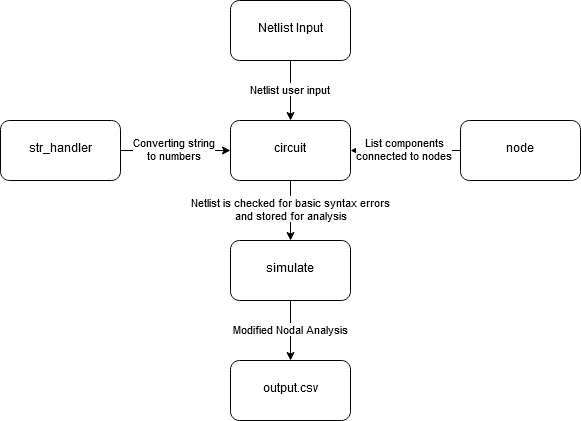
\includegraphics[scale=0.5]{Flow chart.PNG}
		\caption{General flowchart of program}
	\end{figure}
	\textit{circuit} file forms the central section of the program, handling the input of the file and 
	storing it in a form that allows the \textit{simulate} file to perform Transient Analysis on it and outputs
	the file in the format (.CSV) specified by the client.
	\par
	The theoretical information and program design for each of the main files are discussed in the following 
	sections.
	\pagebreak
	\subsection{Components files}
	Due to the OOP design methodology, each component and its necessary functions are described in its own
	respective file. The file \textit{edge.hpp} is the base from which all other circuit components are derived
	from the \textbf{components} folder. 
	\subsection{\textit{str handler.hpp} file}
	The \textit{str handler} file manages all string-related functions. The main function is the  
	\subsection{\textit{node.hpp} file}
	As a circuit can be expressed as a Network Graph, containing branches and edges
	\pagebreak
	\subsection{Circuit.cpp}
	\pagebreak
	\subsection{Simulate.cpp}
	\pagebreak

\section{Testing}
\pagebreak

\section{Optimisations}
\subsection{Sparse Matrices}
\pagebreak

\section{Adding on}
\pagebreak

\section{Appendix}
\subsection{Belbin Roles}
\begin{figure} [h!]
	\centering
	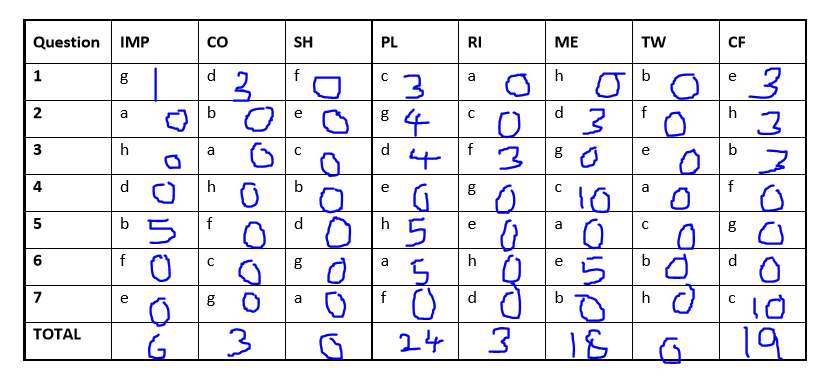
\includegraphics[scale=0.5]{Adam.PNG}
	\caption{Belbin Roles of Adam Rehman}
\end{figure}
\begin{figure} [h!]
	\centering
	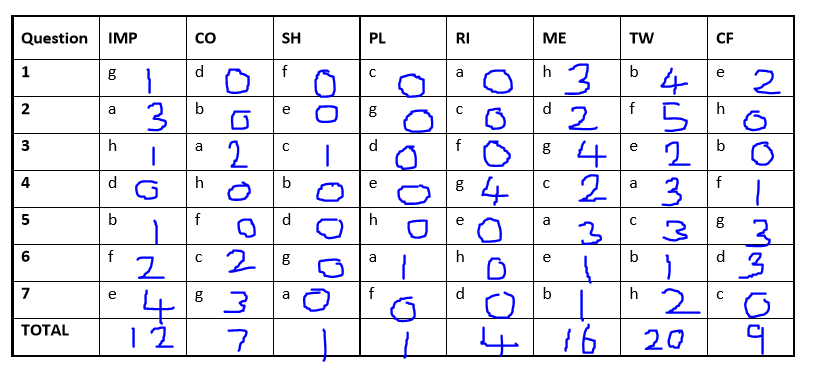
\includegraphics[scale=0.5]{Brandon.PNG}
	\caption{Belbin Roles of Brandon Cann}
\end{figure}
\begin{figure} [h!]
	\centering
	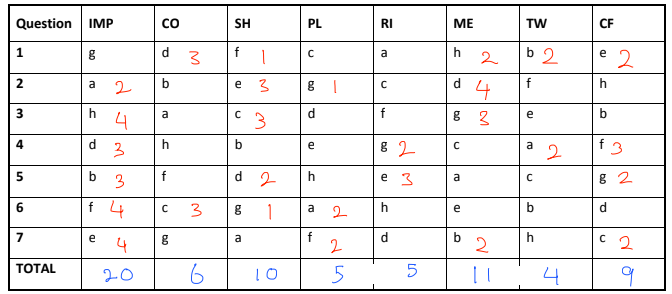
\includegraphics[scale=0.75]{Xin.PNG}
	\caption{Belbin Roles of Xin Wang}
\end{figure}
\pagebreak

\section{References}
\printbibliography[title={References}]
\end{document}